%TC:ignore

\thispagestyle{plain}

\chapter{Ethics Submission}
\label{appendix:ethics}

%This appendix includes a copy of the ethics submission for the project. After you have completed your Ethics submission, you will receive a PDF with a summary of the comments. That document should be embedded in this report, either as images, an embedded PDF or as copied text. The content should also include the Ethics Application Number that you receive.

\textbf{Ethics Application Number: 3958}
  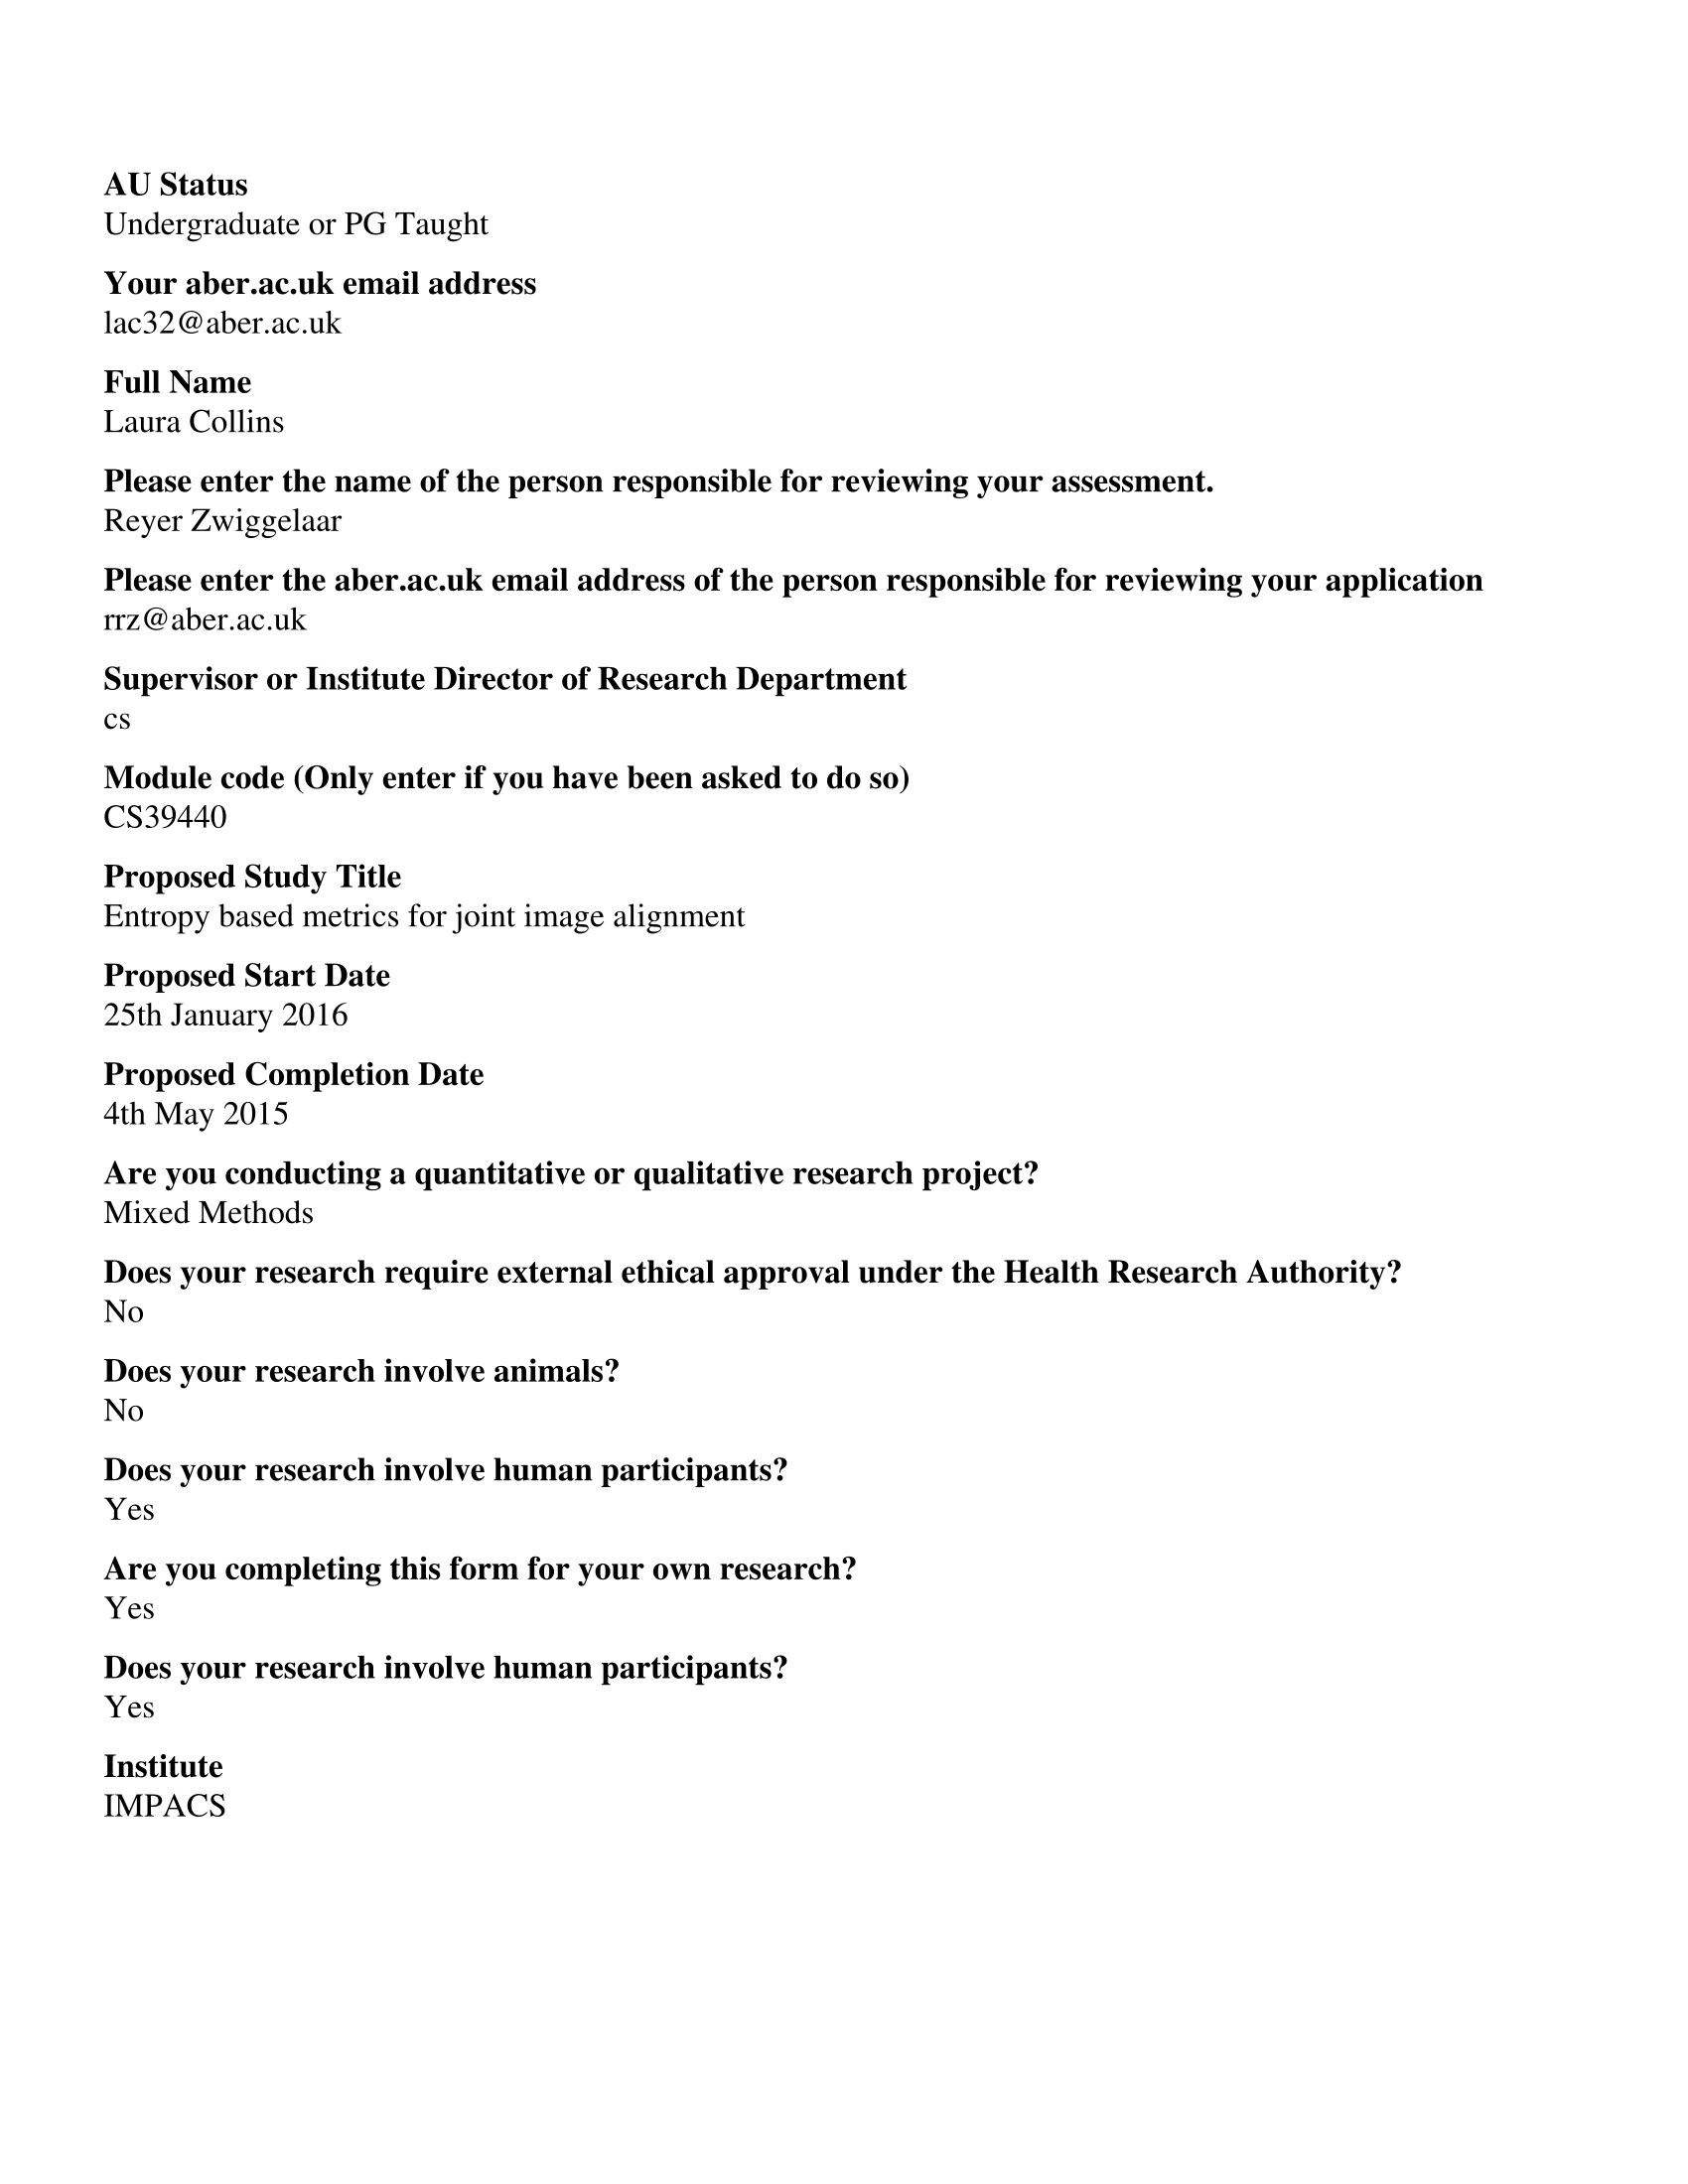
\includegraphics[scale = 0.4,clip,trim=10mm 25mm 25mm 18mm]{Appendix2/3958-1.png}
  %\includepdf[pages=2-3, scale = 0.7,pagecommand={\thispagestyle{plain}}]{Appendix2/3958.pdf}
  \newpage
  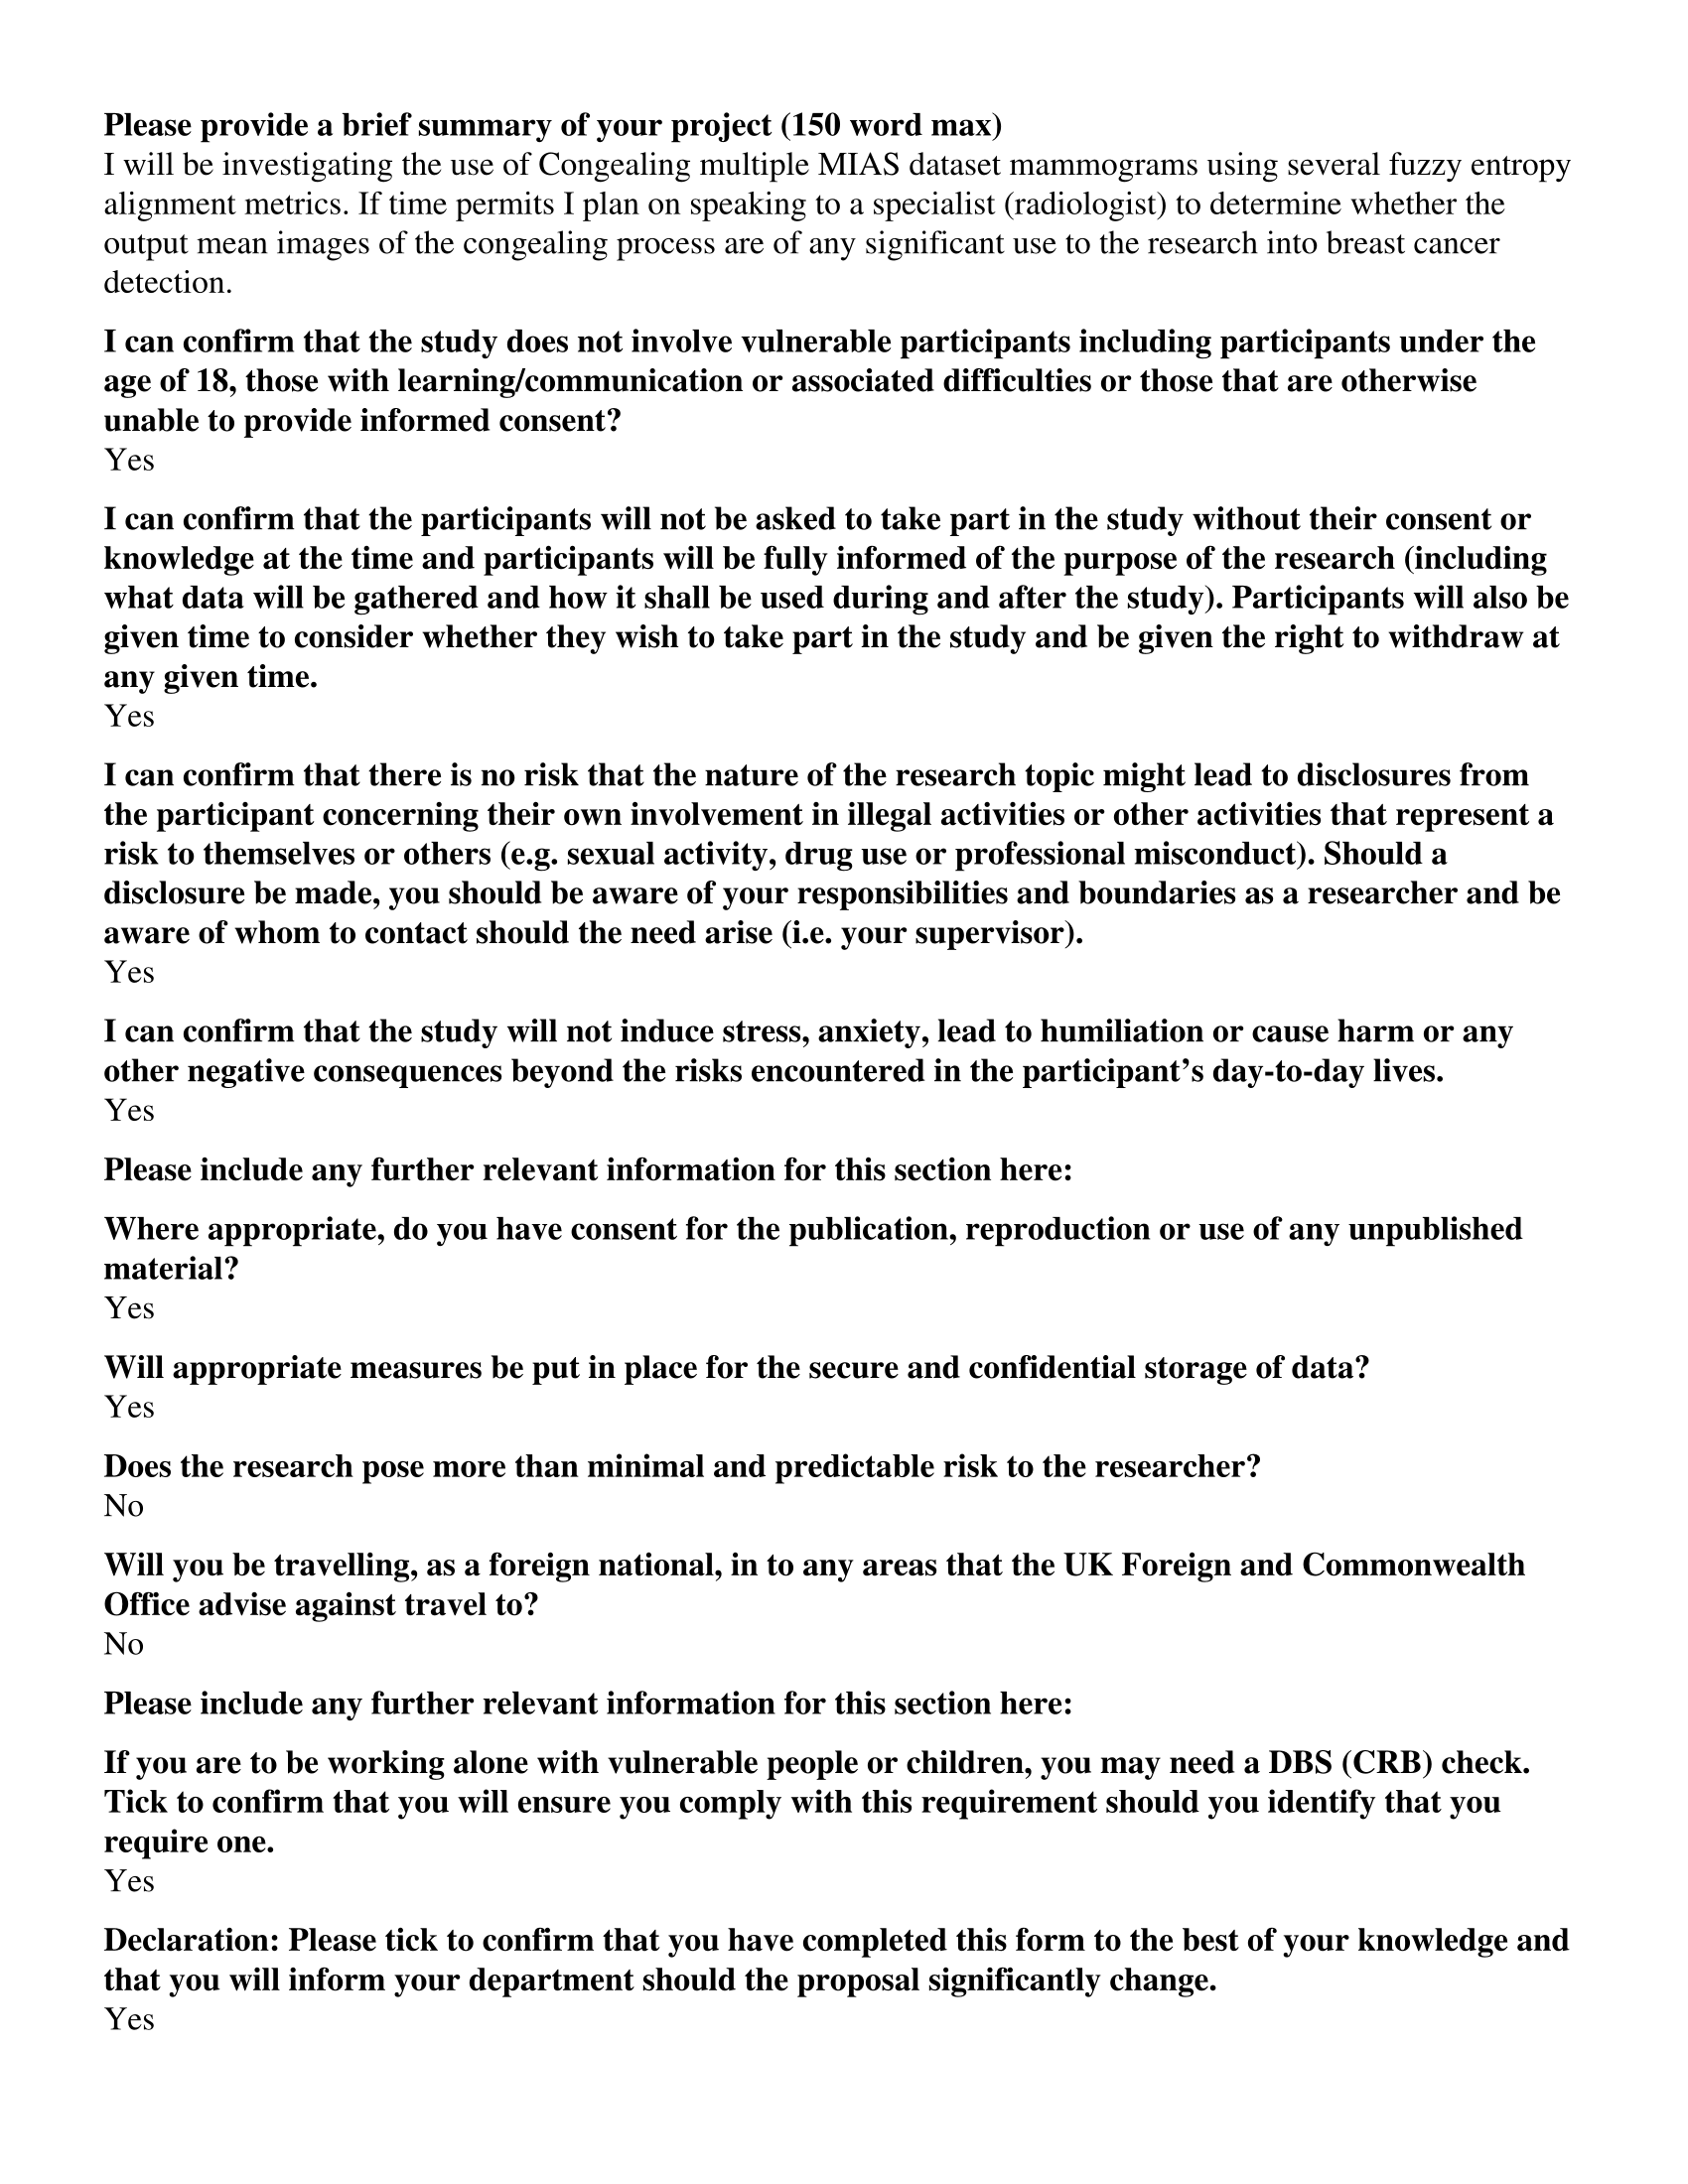
\includegraphics[scale=0.4]{Appendix2/3958-2.png}
  \newpage
  
\includegraphics[scale=0.4]{Appendix2/3958-3.png}

\iffalse
\noindent \textbf{AU Status}
Undergraduate or PG Taught

\noindent \textbf{Your aber.ac.uk email address}
lac32@aber.ac.uk

\noindent \textbf{Full Name}
Laura Collins

\noindent \textbf{Please enter the name of the person responsible for reviewing your assessment.}
Reyer Zwiggelaar

\noindent \textbf{Please enter the aber.ac.uk email address of the person responsible for reviewing your application}
rrz@aber.ac.uk

\noindent \textbf{Supervisor or Institute Director of Research Department}
cs

\noindent \textbf{Module code (Only enter if you have been asked to do so)}
CS39440

\noindent \textbf{Proposed Study Title}
Entropy based metrics for joint image alignment

\noindent \textbf{Proposed Start Date}
25th January 2016

\noindent \textbf{Proposed Completion Date}
4th May 2015

\noindent \textbf{Are you conducting a quantitative or qualitative research project?}
Mixed Methods

\noindent \textbf{Does your research require external ethical approval under the Health Research Authority?}
No

\noindent \textbf{Does your research involve animals?}
No

\noindent \textbf{Does your research involve human participants?}
Yes

\noindent \textbf{Are you completing this form for your own research?}
Yes

\noindent \textbf{Does your research involve human participants?}
Yes

\noindent \textbf{Institute}
IMPACS

\noindent \textbf{Please provide a brief summary of your project (150 word max)}
I will be investigating the use of Congealing multiple MIAS dataset mammograms using several fuzzy entropy alignment metrics. If time permits I plan on speaking to a specialist (radiologist) to determine whether the output mean images of the congealing process are of any significant use to the research into breast cancer detection.

\noindent \textbf{I can confirm that the study does not involve vulnerable participants including participants under the age of 18, those with learning/communication or associated difficulties or those that are otherwise unable to provide informed consent?}
Yes

\noindent \textbf{I can confirm that the participants will not be asked to take part in the study without their consent or knowledge at the time and participants will be fully informed of the purpose of the research (including what data will be gathered and how it shall be used during and after the study). Participants will also be given time to consider whether they wish to take part in the study and be given the right to withdraw at any given time.}
Yes

\noindent \textbf{I can confirm that there is no risk that the nature of the research topic might lead to disclosures from the participant concerning their own involvement in illegal activities or other activities that represent a risk to themselves or others (e.g. sexual activity, drug use or professional misconduct). Should a disclosure be made, you should be aware of your responsibilities and boundaries as a researcher and be aware of whom to contact should the need arise (i.e. your supervisor).}
Yes

\noindent \textbf{I can confirm that the study will not induce stress, anxiety, lead to humiliation or cause harm or any other negative consequences beyond the risks encountered in the participant’s day-to-day lives.}
Yes

\noindent \textbf{Please include any further relevant information for this section here:}

\noindent \textbf{Where appropriate, do you have consent for the publication, reproduction or use of any unpublished material?}
Yes

\noindent \textbf{Will appropriate measures be put in place for the secure and confidential storage of data?}
Yes

\noindent \textbf{Does the research pose more than minimal and predictable risk to the researcher?}
No

\noindent \textbf{Will you be travelling, as a foreign national, in to any areas that the UK Foreign and Commonwealth Office advise against travel to?}
No

\noindent \textbf{Please include any further relevant information for this section here:}

\noindent \textbf{If you are to be working alone with vulnerable people or children, you may need a DBS (CRB) check. Tick to confirm that you will ensure you comply with this requirement should you identify that you require one.}
Yes

\noindent \textbf{Declaration: Please tick to confirm that you have completed this form to the best of your knowledge and that you will inform your department should the proposal significantly change.}
Yes

\noindent \textbf{Please include any further relevant information for this section here:}

\fi
%TC:endignore
